\documentclass[11pt,twoside,a4paper]{article}
% http://www-h.eng.cam.ac.uk/help/tpl/textprocessing/latex_maths+pix/node6.html symboles de math
% http://fr.wikibooks.org/wiki/Programmation_LaTeX Programmation latex (wikibook)
%=========================== En-Tete =================================
%--- Insertion de paquetages (optionnel) ---
%--- Insertion de paquetages (optionnel) ---
\usepackage[french]{babel}   % pour dire que le texte est en fran{\'e}ais
\usepackage{a4}	             % pour la taille   
\usepackage[T1]{fontenc}     % pour les font postscript
\usepackage{epsfig}          % pour gerer les images
%\usepackage{psfig}
\usepackage{amsmath, amsthm} % tres bon mode mathematique
\usepackage{amsfonts,amssymb}% permet la definition des ensembles
\usepackage{float}           % pour le placement des figure
\usepackage{verbatim}


\usepackage{longtable} % pour les tableaux de plusieurs pages

\usepackage[table]{xcolor} % couleur de fond des cellules de tableaux

\usepackage{lastpage}

\usepackage{multirow}

\usepackage{multicol} % pour {\'e}crire dans certaines zones en colonnes : \begin{multicols}{nb colonnes}...\end{multicols}

%% https://texblog.org/2011/02/26/generating-dummy-textblindtext-with-latex-for-testing/
%% https://fr.sharelatex.com/learn/Multiple_columns
%% \usepackage{blindtext}
%% \usepackage{lipsum}
\usepackage{wrapfig}

% \usepackage[top=1.5cm, bottom=1.5cm, left=1.5cm, right=1.5cm]{geometry}
% gauche, haut, droite, bas, entete, ente2txt, pied, txt2pied
\usepackage{vmargin}
\setmarginsrb{1.0cm}{1.0cm}{1.0cm}{1.0cm}{15pt}{3pt}{57pt}{3pt}

\usepackage{lscape} % changement orientation page
\usepackage{pdflscape}
% --- style de page (pour les en-tete) ---
% \pagestyle{headings}
\pagestyle{empty}

% % % en-tete et pieds de page configurables : fancyhdr.sty

% http://www.trustonme.net/didactels/250.html

% http://ww3.ac-poitiers.fr/math/tex/pratique/entete/entete.htm
% http://www.ctan.org/tex-archive/macros/latex/contrib/fancyhdr/fancyhdr.pdf
% \usepackage{fancyhdr}
% \pagestyle{fancy}
% % \newcommand{\chaptermark}[1]{\markboth{#1}{}}
% % \newcommand{\sectionmark}[1]{\markright{\thesection\ #1}}
% \fancyhf{}
% \fancyhead[LE,RO]{\bfseries\thepage}
% \fancyhead[LO]{\bfseries\rightmark}
% \fancyhead[RE]{\bfseries\leftmark}
% \fancyfoot[LE]{\thepage /\pageref{LastPage} \hfill
	% TITLE
% \hfill 
\includegraphics[width=0.5cm]{img/logo_glider.png} }
% \fancyfoot[RO]{
\includegraphics[width=0.5cm]{img/logo_glider.png} \hfill
	% TITLE
% \hfill \thepage /\pageref{LastPage}}
% \renewcommand{\headrulewidth}{0.5pt}
% \renewcommand{\footrulewidth}{0.5pt}
% \addtolength{\headheight}{0.5pt}
% \fancypagestyle{plain}{
	% \fancyhead{}
	% \renewcommand{\headrulewidth}{0pt}
% }

%--- Definitions de nouvelles commandes ---
\newcommand{\N}{\mathbb{N}} % les entiers naturels

%============================= Corps =================================
\begin{document}
\begin{landscape}

% \setcounter{page}{0}
% \thispagestyle{empty}

\setlength\parindent{0cm} %% \noindent

%% https://www.jmdoudoux.fr/java/dej/chap-spring.htm
%% https://javaetmoi.developpez.com/tutoriels/spring/configurez-spring-java/
%% 

\begin{multicols}{2}
	\section*{Memento Spring Framework}
	
	Une vingtaine de modules, 6 briques...
	\begin{itemize}
		\item Core Container (BeanFactory...)
		\item AOP : Aspect Oriented Programmation (fonctions transverses)
		\item Data Access / Data Integration (JDBC, acc{\`e}s aux donn{\'e}es, gestion connexions et gestion des erreurs)
		\item Instrumentation
		\item Test
		\item Web
	\end{itemize} %% ~\\
	
	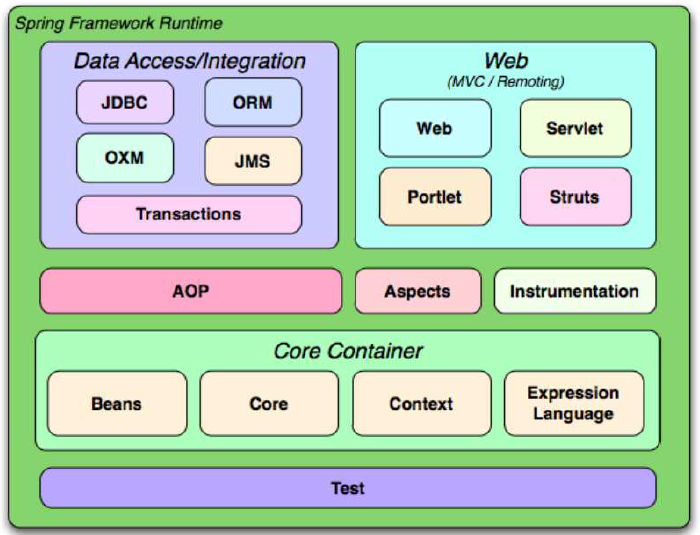
\includegraphics[width=0.95\linewidth]{./SpringFrameworkRuntime.png}~\\
	\emph{\footnotesize Vue d'ensemble du Framework Spring}
	
	%% \begin{figure}[h] %% \begin{wrapfigure}{l}{width=0.95\linewidth}
	%% 	\centering
	%% 	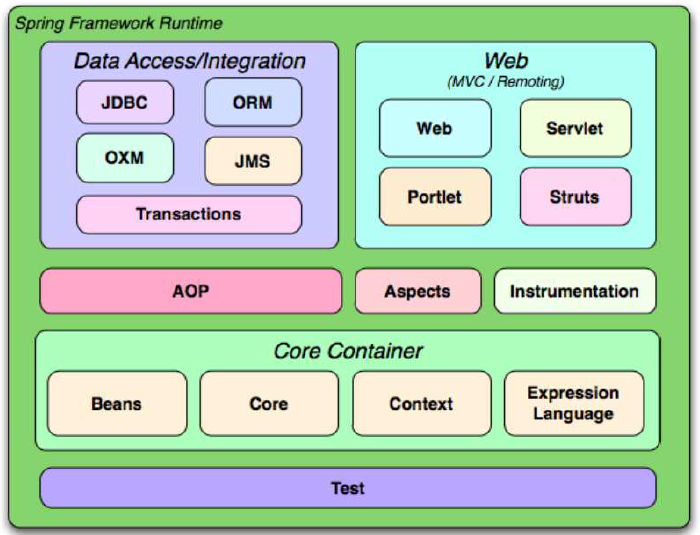
\includegraphics[width=0.95\linewidth]{./SpringFrameworkRuntime.png}
	%% 	\caption{Vue d'ensemble du Framework Spring}
	%% \end{figure} %% \end{wrapfigure}~\\
	
	L'inversion de Contr{\^o}le (IoC) : <<Ne nous appelez pas, nous vous appellerons !>>
	\begin{itemize}
		\item Container configurable
		\item Injection des d{\'e}pendances
		\item Simplification et reconfiguration externe
	\end{itemize}~\\
	
	\vfill
	\columnbreak
	
	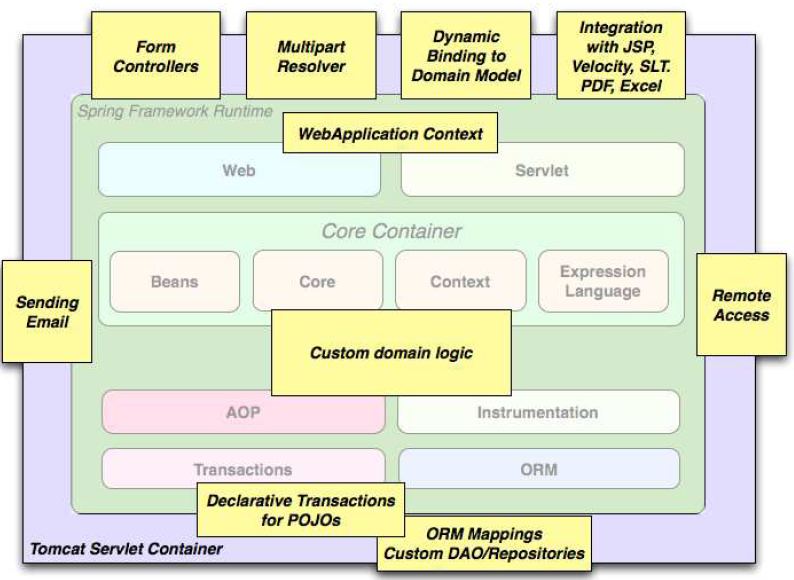
\includegraphics[width=0.90\linewidth]{./SpringFrameworkRuntimeUsage.png}~\\
	\emph{\footnotesize Usages des {\'e}l{\'e}ments du Framework Spring}
	
	\vfill
	
	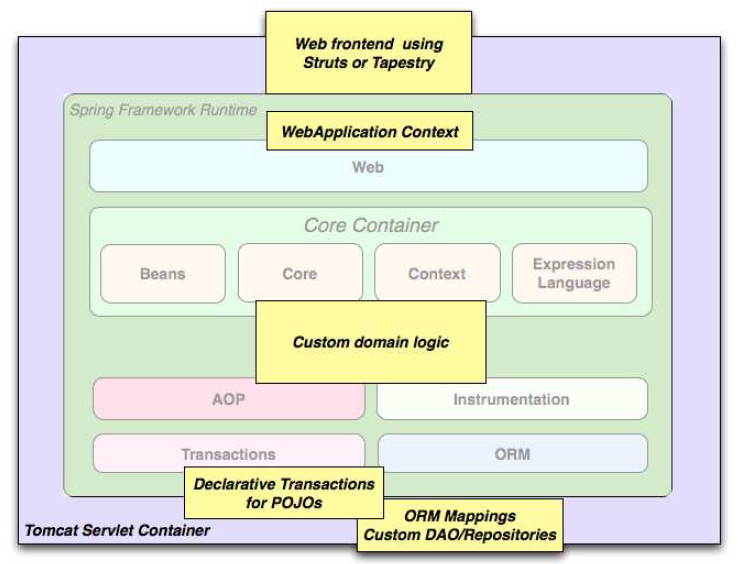
\includegraphics[width=0.90\linewidth]{./SpringFrameworkRuntimeUsageHibernate.png}~\\
	\emph{\footnotesize Usage du Framework Spring avec Hibernate}
	
	% \begin{wrapfigure}{l}{0pt}
		% 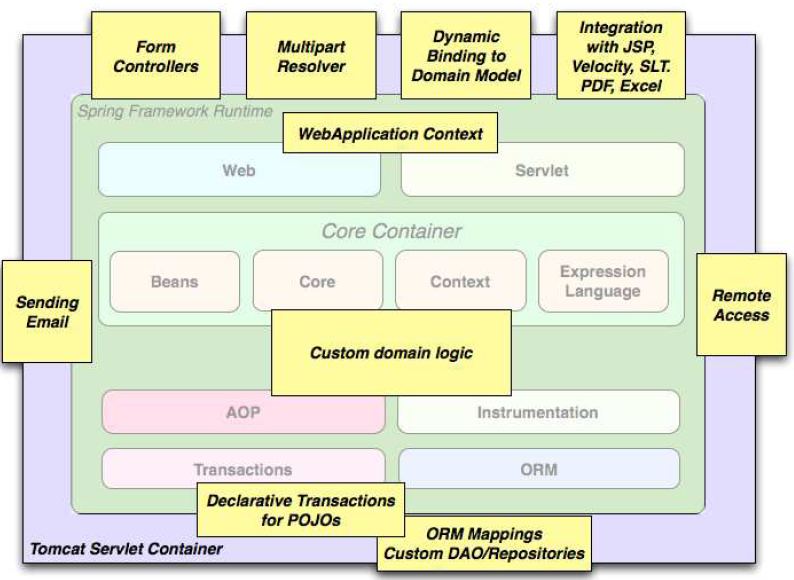
\includegraphics[width=0.95\linewidth]{./SpringFrameworkRuntimeUsage.png}
		% \caption{Usages des {\'e}l{\'e}ments du Framework Spring}
	% \end{wrapfigure}
	
	% \begin{wrapfigure}{l}{0pt}
		% 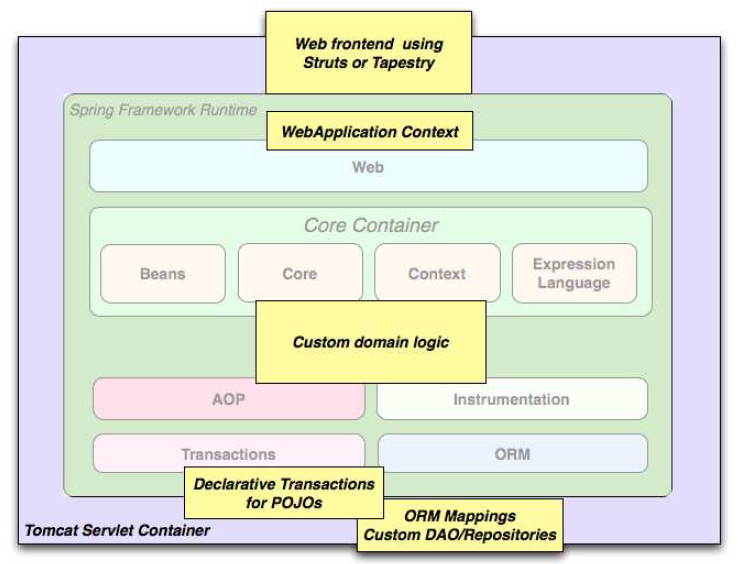
\includegraphics[width=0.95\linewidth]{./SpringFrameworkRuntimeUsageHibernate.png}
		% \caption{Usage du Framework Spring avec Hibernate}
	% \end{wrapfigure}
	
	%% \columnbreak
	%% \vfill
	%% ...
	
	\vfill
	\columnbreak
	
	Conteneur l{\'e}ger de Spring : 
	\begin{itemize}
		\item Gestion des objets applicatifs (Beans) et de leur cycle de vie
		\item Contexte d'application
		\item Annotations
	\end{itemize}~\\
	
	Objects / Classes importantes : 
	\begin{itemize}
		\item Bean (POJO : Plain Old Java Object), g{\'e}r{\'e} par le conteneur
		\item BeanFactory (acc{\`e}s conteneur, peut {\^e}tre cr{\'e}{\'e}e)
		\item ApplicationContext (fabrique et registre Bean's), {\'e}tend BeanFactory, contexte
		\begin{itemize}
			\item m{\'e}thodes fabriques de beans
			\item support messages et internationalisation
			\item support chargememnt fichiers locaux / distants
			\item g{\'e}n{\'e}ration {\'e}v{\`e}nements pour les beans
			\item hi{\'e}rarchisation informations disponibles pour les beans
		\end{itemize}
	\end{itemize}~\\
	
	Fichier de Configuration (XML) : 
	\begin{itemize}
		\item Accès via contexte
		\item \texttt{BeanFactory ctx =~\\
			new ClassPathXmlApplicationContext("spring.xml");}
	\end{itemize}~\\

%% \fbox{ %% \framebox[\textwidth]{%
	\footnotesize
	\begin{verbatim}
<?xml version="1.0" encoding="UTF-8"?>
<beans xmlns="http://www.springframework.org/schema/beans"
    xmlns:xsi="http://www.w3.org/2001/XMLSchema-instance"
    xmlns:p="http://www.springframework.org/schema/p"
    xmlns:aop="http://www.springframework.org/schema/aop"
    xmlns:lang="http://www.springframework.org/schema/lang"
    xmlns:context="http://www.springframework.org/schema/context"
    xsi:schemaLocation="http://www.springframework.org/schema/beans
    http://www.springframework.org/schema/beans/spring-beans.xsd">

</beans>
	\end{verbatim}
	\normalsize
%% } %% framebox
	
	%% \vfill
	%% \columnbreak
	
Quelques exemples de configuration : 
	
	\footnotesize
	\begin{verbatim}
<context:annotation-config />

<context:component-scan base-package="package.impl.beans" />

<bean class="package.to.class.ParentTraceur" />

<bean name="logAd" class="package.aop.Traceur" />
<aop:config>
    <aop:pointcut id="sondesPointCut" 
        expression="execution(int package.impl.*.getValeur())" />
    <aop:advisor advice-ref="logAd" pointcut-ref="sondesPointCut" />
</aop:config>
<aop:aspectj-autoproxy />
<bean id="traceurAspect" class="package.aop.TraceurAspect" />

<bean name="messageSource"
        class="org.springframework.context.support.ResourceBundleMessageSource">
    <property name="basename" value="messages" />
</bean>

<bean id="beanEmetteur" 
        class="package.impl.EmetteurAlerteConsoleSansRepetition" 
        scope="prototype" />
<!-- scope="prototype||singleton" -->

<bean id="beanSonde" class="package.impl.SondeCompteurFichier">
    <property name="repertoire" value="c:/temp" />
</bean>

<bean id="beanSondeUsage" class="package.impl.SondeUsageDisque">
    <property name="disque" value="c:" />
</bean>

<bean id="beanSondeDetect" class="package.impl.SondeDetectionFichier">
    <constructor-arg value="c:/temp/test.txt" />
    <constructor-arg value="true" />
</bean>

<bean id="surveillanceDefaut" 
        class="package.spring.SystemeDeSurveillance" 
        abstract="true">
    <property name="frequence" value="5" />
    <property name="seuil" value="20" />
</bean>

<bean id="beanSondeTemp" class="package.spring.impl.SondeFactory"
    factory-method="creerSondeTemp" />

<bean id="beanSondeDisque1" class="package.spring.impl.SondeUsageMultiDisques">
    <property name="disques">
        <array>
            <value>C:</value>
            <value>E:</value>
        </array>
        <!-- same for list, set, map, props -->
    </property>
</bean>

<bean id="beanSondeDisque2" class="package.spring.impl.SondeUsageMultiDisques">
    <property name="disques" value="C:,E:" />
    <!-- only values (not references !) -->
</bean>

<!-- <bean id="beanSurveillance" parent="surveillanceDefaut" >
    <property name="seuil" value="1" />
    <property name="sonde" ref="beanSondeDisque2" />
    <property name="emetteur" ref="beanEmetteur" />
</bean> -->

<!-- <bean id="beanSurveillance"
    parent="surveillanceDefaut"
    p:seuil="1"
    p:sonde-ref="beanSondeDisque2"
    p:emetteur-ref="beanEmetteur" /> -->

<bean id="beanSurveillance"
    parent="surveillanceDefaut"
    p:seuil="1"
    init-method="demarrer"
    destroy-method="arreter" />
    <!-- autowire="byName" -->

<alias name="beanSondeDisque2" alias="sonde" />
<alias name="beanEmetteur" alias="emetteur" />

<lang:groovy id="sondeGroovy"
        script-source="testSonde.groovy" refresh-check-delay="5">
    <lang:property name="message" value="Passage dans Groovy" />
</lang:groovy>

<bean id="beanSurveillanceMultiple"
        class="package.spring.SystemeDeSurveillanceMultiple">
    <property name="surveillances">
        <list>
            <ref bean="beanSurveillance" />
            <bean parent="surveillanceDefaut">
                <property name="sonde" ref="sondeGroovy" />
                <property name="emetteur" ref="beanEmetteur" />
            </bean>
        </list>
    </property>
</bean>
	\end{verbatim}
	\normalsize
	
	\vfill
	\columnbreak
	
	...
	
\end{multicols}

\clearpage

\end{landscape}
\end{document}
